\documentclass[border=1mm]{standalone}
% \usepackage[margin=2.5cm]{geometry}

\usepackage{graphicx,tikz,tikz-layers,amsmath,ifthen,tabularray,xcolor,fontawesome5} 
\usetikzlibrary{decorations.markings,calc,positioning,arrows,shapes.geometric,arrows.meta,matrix,decorations.text}

\colorlet{myred}{red!80!black}
\colorlet{myblue}{blue!80!black}
\colorlet{mybluee}{myblue!80!black}
\colorlet{mygreen}{green!60!black}
\colorlet{myorange}{orange!70!red!60!black}
\colorlet{mydarkred}{red!20!black}
\colorlet{mydarkblue}{blue!40!black}
\colorlet{mydarkgreen}{green!20!black}




\begin{document}

% \resizebox{\textwidth}{!}{
\tikz[font=\small, scale=1, every node/.style={outer sep=0pt, inner sep=0pt, rounded corners=.5mm, align=center}, w/.style={minimum width=#1}, h/.style={minimum height=#1}, s/.style={minimum size=#1}, eu/.style={shorten >=#1}, ed/.style={shorten <=#1}, line join=round]
{
\tikzset{>={Latex[length=1.5mm, width=1.25mm]}}

\foreach \i in {1,2,...,9}
\node[draw, w=.8cm, h=.4cm, fill=gray!15] (\i) at (\i,0) {};

   \foreach \i/\j in {3/A,4/small,5/red,6/boat,7/on,8/the,9/water} {%
        \ifnum\i<7
            \node[w=.8cm, h=.45cm, text=gray!50] (a\i) at (\i,2.5) {\strut \j};  
        \else
            \node[w=.8cm, h=.45cm, text=black] (a\i) at (\i,2.5) {\j};  
        \fi
    }

\foreach \i\j in {3/A,4/small,5/red,6/\color{gray!50}boat,7/\color{gray!50}on,8/\color{gray!50}the,9/\color{gray!50}water}
\node[w=.8cm, h=.45cm] (b\i) at (\i,-3.85) {\strut \j};

\node[draw, w=8.8cm, h=.95cm, fill=myblue!15, anchor=south east] (a) at ($(9.north east)+(0,.5)$) {\textbf{Language Model}\\Self Attention Layers};

\node[draw, w=6.8cm, h=.95cm, fill=mygreen!15, anchor=north east] (b) at ($(9.south east)+(0,-.5)$) {\textbf{Language Model}\\Text Embedder};

\node[draw, w=1.8cm, h=.95cm, fill=mygreen!15, anchor=north west] (c) at ($(1.south west)+(0,-.5)$) {Vision\\Encoder};

% Arrows
\foreach \i in {3,4,...,9}{
\ifnum\i>5
\draw[->, gray!50] (b\i.north)--(b\i.north|-b.south);
\else
\draw[->] (b\i.north)--(b\i.north|-b.south);
\fi
}

\foreach \i in {3,4,...,9}{
\ifnum\i<7
\draw[<-, gray!50] (a\i.south)--(a\i.south|-a.north);
\else
\draw[<-] (a\i.south)--(a\i.south|-a.north);
\fi}

\foreach \i in {1,2,...,9}
\draw[->] (\i.north)--(\i.north|-a.south);

\foreach \i in {3,4,...,9}
\draw[<-] (\i.south)--(\i.south|-b.north);

\draw[<-] (1.south)--(1.south|-c.north);
\draw[<-] (2.south)--(2.south|-c.north);

\node[below=.5cm of c] (ph) {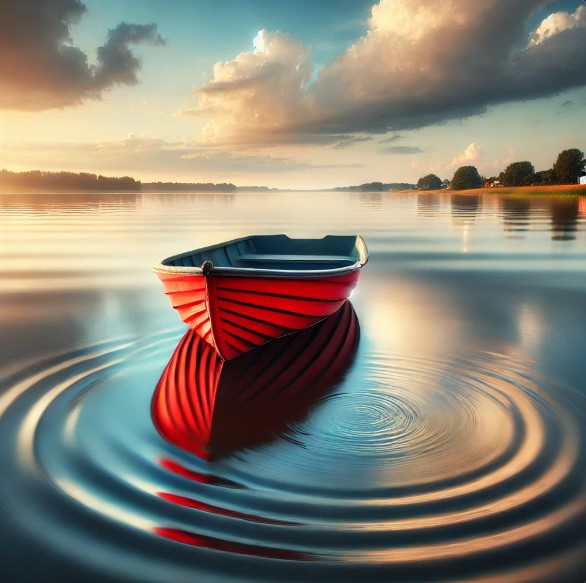
\includegraphics[width=1.8cm]{images/redboat.jpg}};

\draw[->, myred] (a9.-50)--(a9.-50|-a.north);
\draw[->, myred] (a8.-50)--(a8.-50|-a.north);
\draw[->, myred] (a7.-50)--(a7.-50|-a.north);
\draw[<-, myred] (1.50)--(1.50|-a.south);
\draw[<-, myred] (2.50)--(2.50|-a.south);
\draw[->, myred] (1.-50)--(1.-50|-c.north);
\draw[->, myred] (2.-50)--(2.-50|-c.north);

\draw[->] (ph)--(c);

\node[gray, anchor=east] at ($(b.east)+(-.2,0)$) {\footnotesize\faSnowflake$\:$Frozen};
\node[gray, anchor=east] at ($(a.east)+(-.2,0)$) {\footnotesize\faSnowflake$\:$Frozen};

\node[gray, anchor=west] at ($(b.west)+(.2,0)$) {\footnotesize$g(\theta)$};
\node[gray, anchor=west] at ($(a.west)+(.2,0)$) {\footnotesize$f(\theta)$};
\node[gray, anchor=east] at ($(c.east)+(-.05,0.3)$) {\scriptsize$v(\!\phi\!)$};
}

% }



\end{document}
